\section{Resultados} % Seções são adicionadas para organizar sua apresentação em blocos discretos, todas as seções e subseções são automaticamente exibidas no índice como uma visão geral da apresentação, mas NÃO são exibidas como slides separados.

%----------------------------------------------------------------------------------------

\begin{frame}
    \frametitle{Sumarização}
    \only<1>{
        \begin{table}[htbp]
            \centering
                \begin{tabular}{l c c}
                \hline
                Dimensão de Qualidade & Valor Médio & DP Médio\\
                \hline
                Consistência (AH) & 2.39 & 0.87\\
                Naturalidade (AH) & 3.58 & 0.97\\
                Relevância (AH)   & 2.46 & 0.97\\
                Coerência (AH)    & 2.59 & 0.95\\
                \hline
                \end{tabular}
            \caption{Médias de Avaliações Humanas para a tarefa de Sumarização.}
        \end{table}
    }
    \only<2>{
        \begin{table}
            \centering
            \resizebox{\textwidth}{!}{
                \begin{tabular}{l c c c c}
                    \hline
                    Métrica & Consistência & Naturalidade & Relevância & Coerência \\
                    \hline
                    \hline
                    ROUGE-1 & 0.21 & 0.29 & 0.29 & 0.24\\
                    ROUGE-2 & 0.18 & 0.27 & 0.23 & 0.24\\
                    ROUGE-L & 0.28 & 0.36 & 0.38 & 0.35\\
                    BLEU    & 0.28 & 0.35 & 0.33 & 0.35\\
                    BLEU-1  & 0.31 & 0.28 & 0.28 & 0.27\\
                    BLEU-2  & 0.27 & 0.27 & 0.25 & 0.27\\
                    METEOR  & 0.32 & 0.30 & 0.27 & 0.32\\
                    \hline
                    BERTScore-p  & 0.38 & 0.37 & 0.37 & 0.42\\
                    BERTScore-r  & 0.38 & \textbf{0.40} & 0.40 & 0.39\\
                    BERTScore-f1 & 0.40 & \textbf{0.40} & 0.40 & \textbf{0.43}\\
                    BARTScore    & \textbf{0.42} & 0.38 & \textbf{0.44} & 0.40\\
                    MoverScore   & 0.26 & 0.30 & 0.32 & 0.29\\
                    \hline
                \end{tabular}
            }
            \caption{Valores de Pearson da tarefa de Sumarização.}
        \end{table}
    }
    \only<3>{
        \begin{table}
            \centering
            \begin{tabular}{c l}
                \hline
                Valores de Pearson & Interpretação \\
                \hline
                0.90–1.00 & Muito forte    \\
                0.70–0.89 & Forte          \\
                0.40–0.69 & Moderada       \\
                0.10–0.39 & Fraca          \\
                0.00–0.10 & Negligenciável \\
                \hline
            \end{tabular}
            \caption{Discretização dos valores de Pearson.}
        \end{table}
    }
\end{frame}

%----------------------------------------------------------------------------------------

\begin{frame}
    \frametitle{Question-Answering}
    \only<1>{
        \begin{table}
            \centering
                \begin{tabular}{l c c}
                \hline
                Dimensão de Qualidade & Valor Médio & DP Médio\\
                \hline
                Consistência (AH) & 3.44 & 0.80\\
                Naturalidade (AH) & 4.05 & 0.73\\
                Relevância (AH)   & 3.48 & 0.71\\
                Coerência (AH)    & 3.55 & 0.74\\
                \hline
                \end{tabular}
            \caption{Médias de Avaliações Humanas para a tarefa de QA.}
        \end{table}
    }
    \only<2>{
        \begin{table}
            \centering
            \resizebox{\textwidth}{!}{
                \begin{tabular}{l c c c c}
                    \hline
                    Métrica & Consistência & Naturalidade & Relevância & Coerência \\
                    \hline
                    \hline
                    ROUGE-1 & 0.58 & 0.45 & 0.56 & 0.55\\
                    ROUGE-2 & 0.50 & 0.33 & 0.51 & 0.49\\
                    ROUGE-L & 0.56 & 0.44 & 0.55 & 0.54\\
                    BLEU    & 0.43 & 0.24 & 0.44 & 0.43\\
                    BLEU-1  & 0.51 & 0.37 & 0.50 & 0.49\\
                    BLEU-2  & 0.53 & 0.37 & 0.53 & 0.52\\
                    METEOR  & \textbf{0.61} & 0.49 & 0.59 & \textbf{0.59}\\
                    \hline
                    BERTScore-p  & 0.57 & 0.45 & 0.58 & 0.56\\
                    BERTScore-r  & 0.59 & \textbf{0.51} & 0.60 & 0.57\\
                    BERTScore-f1 & 0.60 & 0.50 & \textbf{0.61} & \textbf{0.59}\\
                    BARTScore    & 0.60 & 0.48 & 0.58 & \textbf{0.59}\\
                    MoverScore   & 0.44 & 0.26 & 0.44 & 0.42\\
                    \hline
                \end{tabular}
            }
            \caption{Valores de Pearson da tarefa de Question-Answering.}
        \end{table}
    }
    \only<3>{
        \begin{figure}
            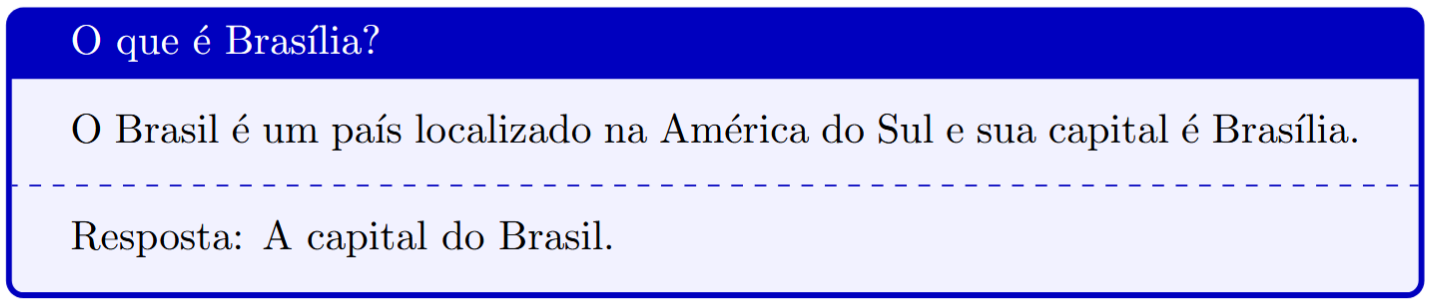
\includegraphics[width=0.9\textwidth]{QA.png}
        \end{figure}
    }
    \only<4>{
        \begin{figure}
            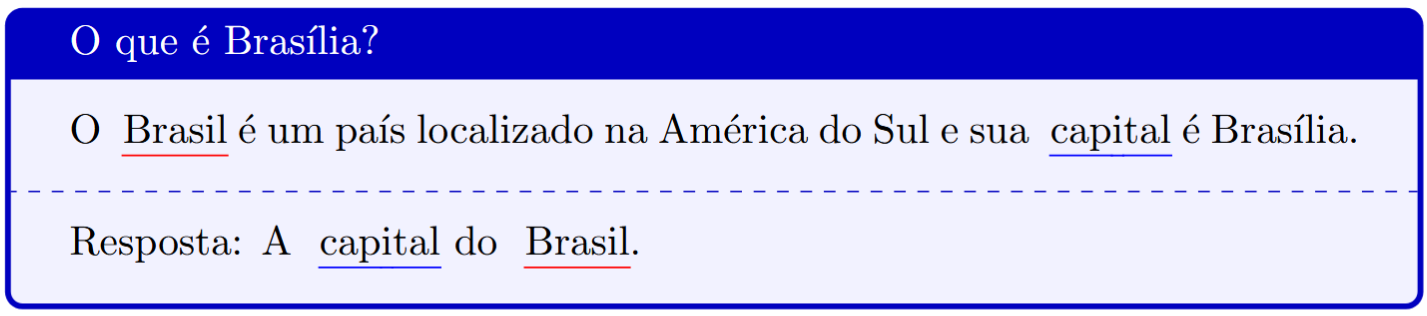
\includegraphics[width=0.9\textwidth]{qa-2.png}
        \end{figure}
    }
    \only<5>{
        \begin{table}
            \centering
            \resizebox{\textwidth}{!}{
                \begin{tabular}{l c c c c}
                    \hline
                    Métrica & Consistência & Naturalidade & Relevância & Coerência \\
                    \hline
                    \hline
                    ROUGE-1 & 0.58 & 0.45 & 0.56 & 0.55\\
                    ROUGE-2 & 0.50 & 0.33 & 0.51 & 0.49\\
                    ROUGE-L & 0.56 & 0.44 & 0.55 & 0.54\\
                    BLEU    & 0.43 & 0.24 & 0.44 & 0.43\\
                    BLEU-1  & 0.51 & 0.37 & 0.50 & 0.49\\
                    BLEU-2  & 0.53 & 0.37 & 0.53 & 0.52\\
                    METEOR  & \textbf{0.61} & 0.49 & 0.59 & \textbf{0.59}\\
                    \hline
                    BERTScore-p  & 0.57 & 0.45 & 0.58 & 0.56\\
                    BERTScore-r  & 0.59 & \textbf{0.51} & 0.60 & 0.57\\
                    BERTScore-f1 & 0.60 & 0.50 & \textbf{0.61} & \textbf{0.59}\\
                    BARTScore    & 0.60 & 0.48 & 0.58 & \textbf{0.59}\\
                    MoverScore   & 0.44 & 0.26 & 0.44 & 0.42\\
                    \hline
                \end{tabular}
            }
            \caption{Valores de Pearson da tarefa de Question-Answering.}
        \end{table}
    }
    \only<6>{
        \begin{table}[htbp]
            \centering
            \begin{tabular}{c l}
                \hline
                Valores de Pearson & Interpretação \\
                \hline
                0.90–1.00 & Muito forte    \\
                0.70–0.89 & Forte          \\
                0.40–0.69 & Moderada       \\
                0.10–0.39 & Fraca          \\
                0.00–0.10 & Negligenciável \\
                \hline
            \end{tabular}
            \caption{Discretização dos valores de Pearson.}
        \end{table}
    }
\end{frame}